%% This document should serve as a base for most mathematically
%% oriented documents. There is probably a better way to do this.

\documentclass[11pt]{article}
%\renewcommand\thesubsection{\thesection.\alph{subsection}}
\usepackage{graphicx, subcaption, amsfonts, amsmath, amsthm, empheq, setspace, lscape}
\captionsetup{width=0.8\textwidth}
\newtheorem*{thm:jnf}{Jordan normal form for square matrices}
% \usepackage[toc,page]{appendix}
%% some new commands I have no idea how they work
\newcommand*\widefbox[1]{\fbox{\hspace{2em}#1\hspace{2em}}}
\newlength\dlf
\newcommand\alignedbox[2]{
  % Argument #1 = before & if there were no box (lhs)
  % Argument #2 = after & if there were no box (rhs)
  &  % Alignment sign of the line
  {
    \settowidth\dlf{$\displaystyle #1$}  
    % The width of \dlf is the width of the lhs, with a displaystyle font
    \addtolength\dlf{\fboxsep+\fboxrule}  
    % Add to it the distance to the box, and the width of the line of the box
    \hspace{-\dlf}  
    % Move everything dlf units to the left, so that & #1 #2 is aligned under #1 & #2
    \boxed{#1 #2}
    % Put a box around lhs and rhs
  }
}
%% end new commands I have no idea how they work

\newcommand\ER{Erd\H{o}s-R\'{e}nyi}
\newcommand{\K}[1]{\mathcal{K}^{#1}}
\newcommand{\Kk}{\mathcal{K}^k}
\newcommand{\Forall}{\; \forall \;}
\newcommand\numberthis{\addtocounter{equation}{1}\tag{\theequation}}
\DeclareMathOperator*{\argmin}{\arg\!\min}
% \captionsetup{labelformat=empty,labelsep=none}
\setlength{\labelsep}{3cm}
\usepackage[top=1in, bottom=1in, left=1in, right=1in]{geometry}
% \setlength{\parindent}{1.5pt}
\graphicspath{ {../figs/} }
\pagestyle{plain}
\begin{document}
% \begin{spacing}{2.2}
% \end{spacing}

% \section{Introduction}

% From geographically distributed power grids to online social media, a wide variety of systems have recently been studied in the framework of complex networks. While the flexibility of this methodology has facilitated its widespread application across different fields, it has also given rise to a vast range of descriptive paradigms such as basic unlabeled, undirected, static networks to dynamic, directed and labeled systems with complicated community structure. In turn, this has led to the development of many disparate methods designed to investigate some small subclass of this large family of problems. It is undoubtedly useful to incorporate system-specific information into network research, but it would also be useful to develop an investigative toolbox broadly applicable across systems. \\
% When faced with a complex network, it is often beneficial to develop some reduced description of the problem that sufficiently captures desired behavior in a reduced number of variables. Identifying this reduced description itself aids in identifying important network features, and it can subsequently be used for more informed, and hopefully more computationally efficient, experimentation. This sort of dimensionality reduction has been found in a range of systems , but again, each problem required its own method of dimensionality reduction...

% Due to the flexibility of this methodology, the actual structure and description of these 

\section{Dimensionality reduction}

Given some dataset $\{x_1, x_2, ..., x_N\}$ in which $x_i \in \mathbb{R}^n$, there are many techniques to uncover some simpler description of the data $\{y_1, y_2, ..., y_N\}$ where $y_i \in \mathbb{R}^p$ and $p \ll n$. The hope is that these new points, lower-dimensional points sufficiently capture, in some mathematically precise sense, the important features of the original data. In essence, we would like to describe our data as concisely as possible.

Perhaps the best-known method for achieving this is principal component analysis (PCA). This method attempts to capture the important features of the data by identifying linear correlations between input variables. Thus, if the three-dimensional input points $x_i \in \mathbb{R}^3$ actually only span a two-dimensional plane, PCA would uncover two basis vectors spanning the plane itself, allowing each of the original three-dimensional points to be efficiently described with two new coordinates. This process is illustrated in Fig. (\ref{fig:pca}).

\begin{figure}[!h]

  \begin{center}
    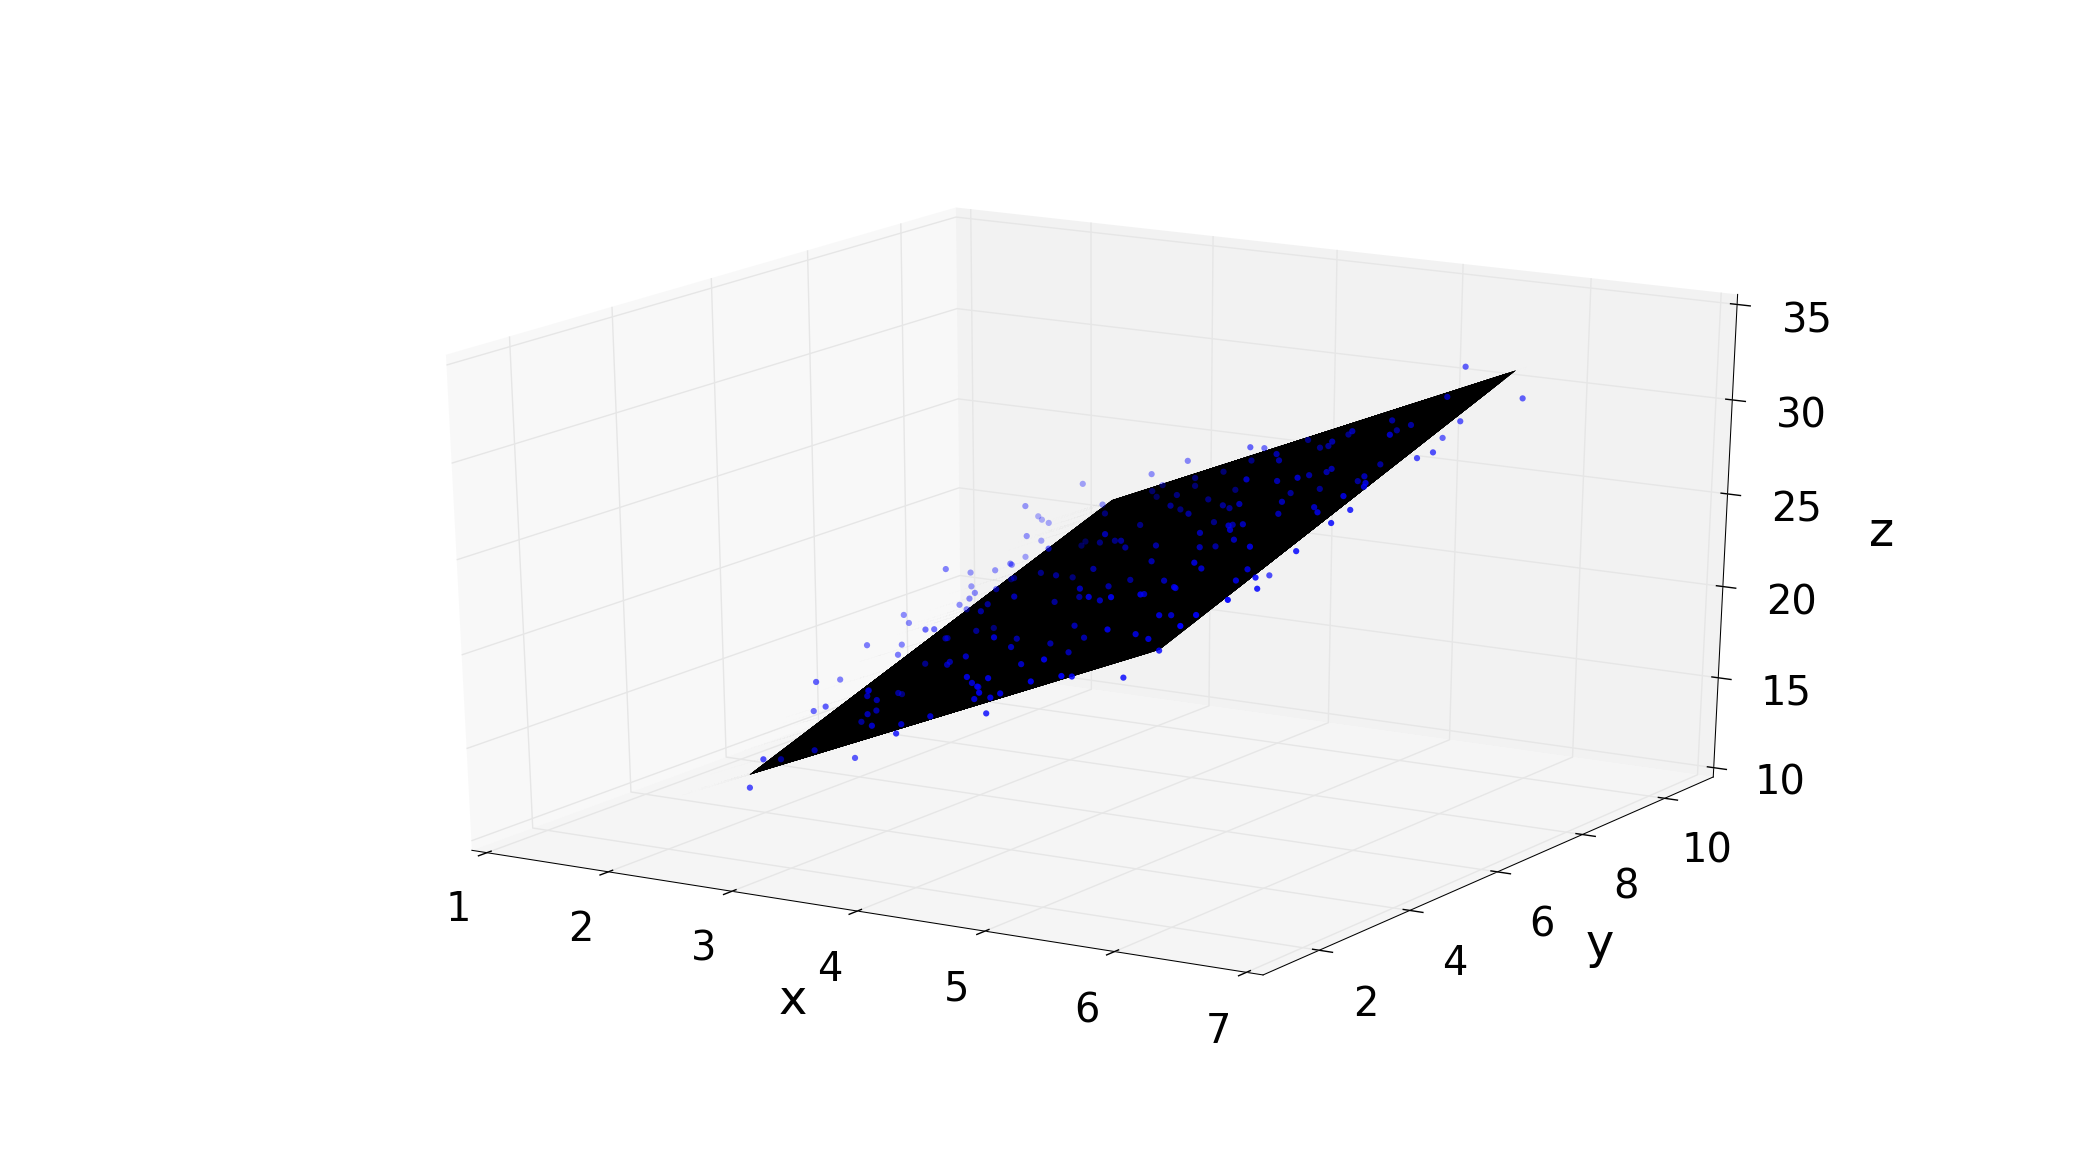
\includegraphics[width=1.0\textwidth]{pca_combined}
    \caption{Three dimensional dataset (blue), and two-dimensional plane uncovered by PCA (black).}
    \label{fig:pca}
  \end{center}

\end{figure}

Unfortunately, as mentioned, this conceptually simple technique assumes the data is well-described by linear relationships between the input variables, whereas datasets generally involve nonlinearities. Thus, in our application we turn to the nonlinear dimensionality reduction technique diffusion maps (DMAPS). Roughly speaking, by simulating a diffusion process over the dataset, DMAPS is able to reveal underlying, low-dimensional nonlinear structure. This is accomplished by calculating approximate eigenfunctions (actually eigenvectors of a Markov matrix, denoted by $\Phi_i$) of the diffusion and subsequently using these eigenvectors to embed the data. This is illustrated in Fig. (\ref{fig:swissroll}), in which the algorithm is applied to a collection of points $\{x_1, x_2, ..., x_N\}$, $x_i \in \mathbb{R}^3$ that lie on a curved plane. The result, shown in Fig. (\ref{fig:swissroll:embedding}) is a concise, two-dimensional embedding of the data into $\{y_1, y_2, ..., y_N\}$, $y_i \in \mathbb{R}^2$, giving us a more efficient description of each point by it's coordinates along the length and width of the underlying plane. Note that PCA would not produce meaningful results in this context, as the relations between input variables are nonlinear.


% \begin{figure}[!h]
%   \begin{subfigure}{.5\textwidth}
%     \begin{center}
%       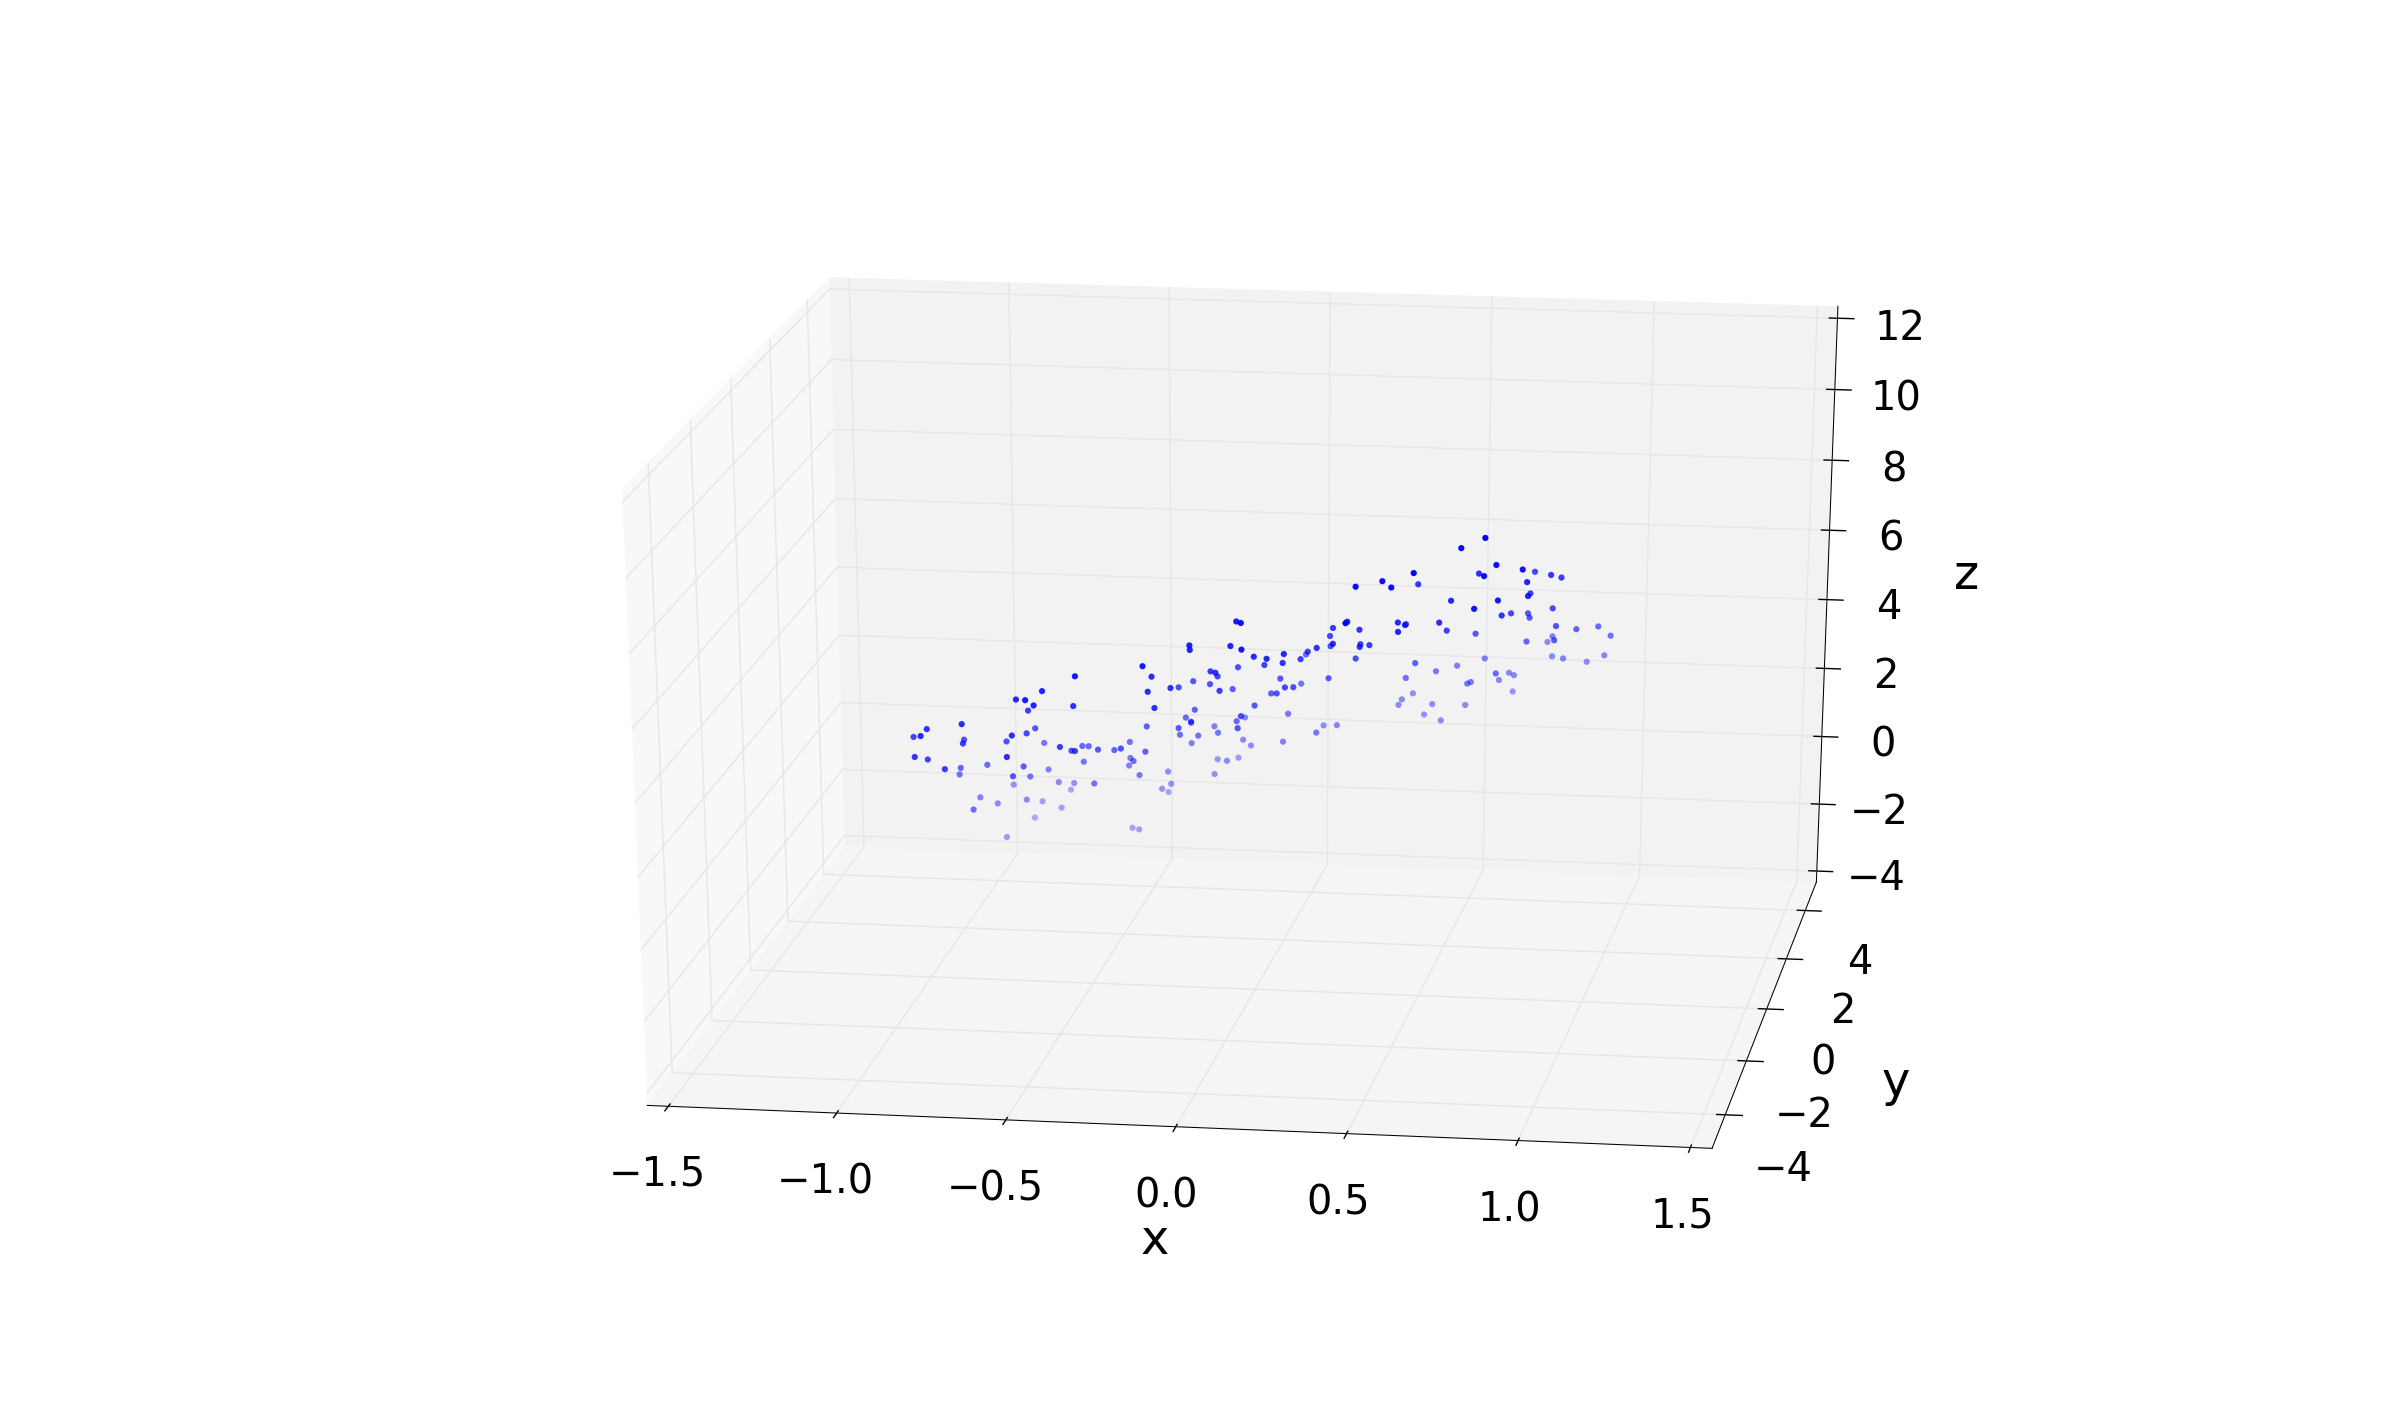
\includegraphics[width=1.2\textwidth]{pca_dataset}
%       \caption{Three dimensional dataset lying on a two dimenisonal plane.}
%       \label{fig:pca:dataset}
%     \end{center}
%   \end{subfigure}
%   \begin{subfigure}{.5\textwidth}
%     \begin{center}
%       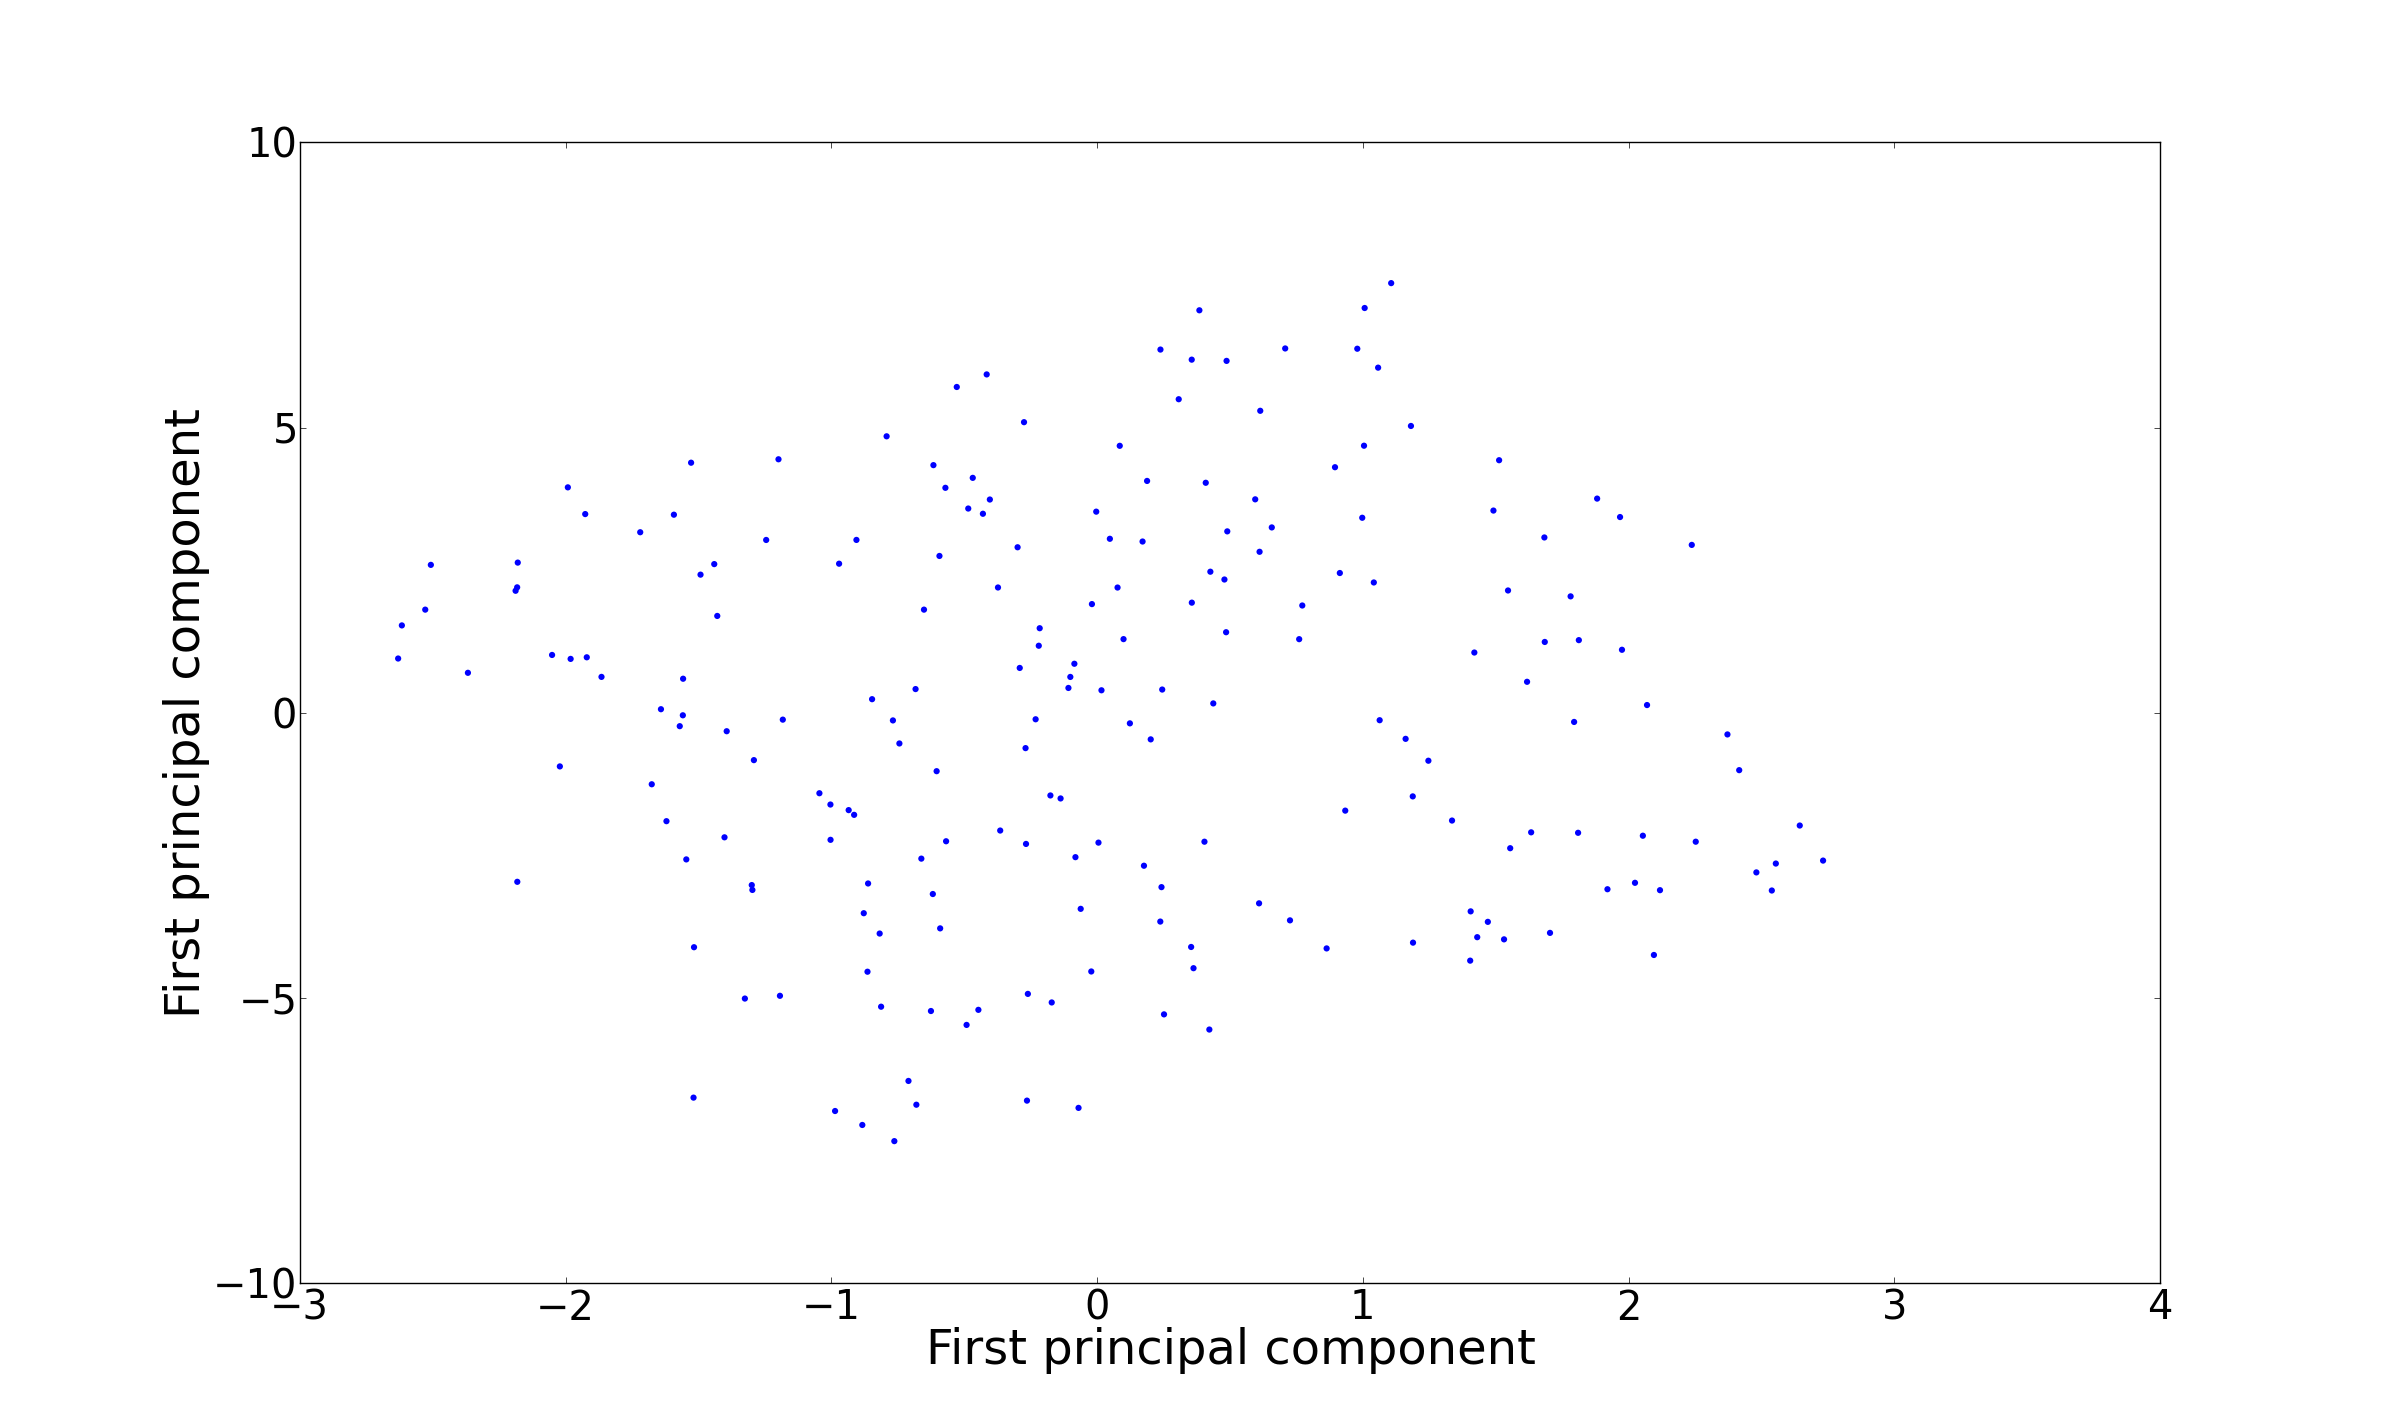
\includegraphics[width=1.0\textwidth]{pca_embedding}
%       \caption{Embedding of data with first two principal components. PCA successfully uncovers the underlying plane.}
%       \label{fig:pca:embedding}
%     \end{center}
%   \end{subfigure}
%   \caption{Illustration of PCA's ability to uncover linear manifolds.}
%   \label{fig:pca}
% \end{figure}

\begin{figure}[!h]
    \begin{center}
  \begin{subfigure}{1.0\textwidth}
      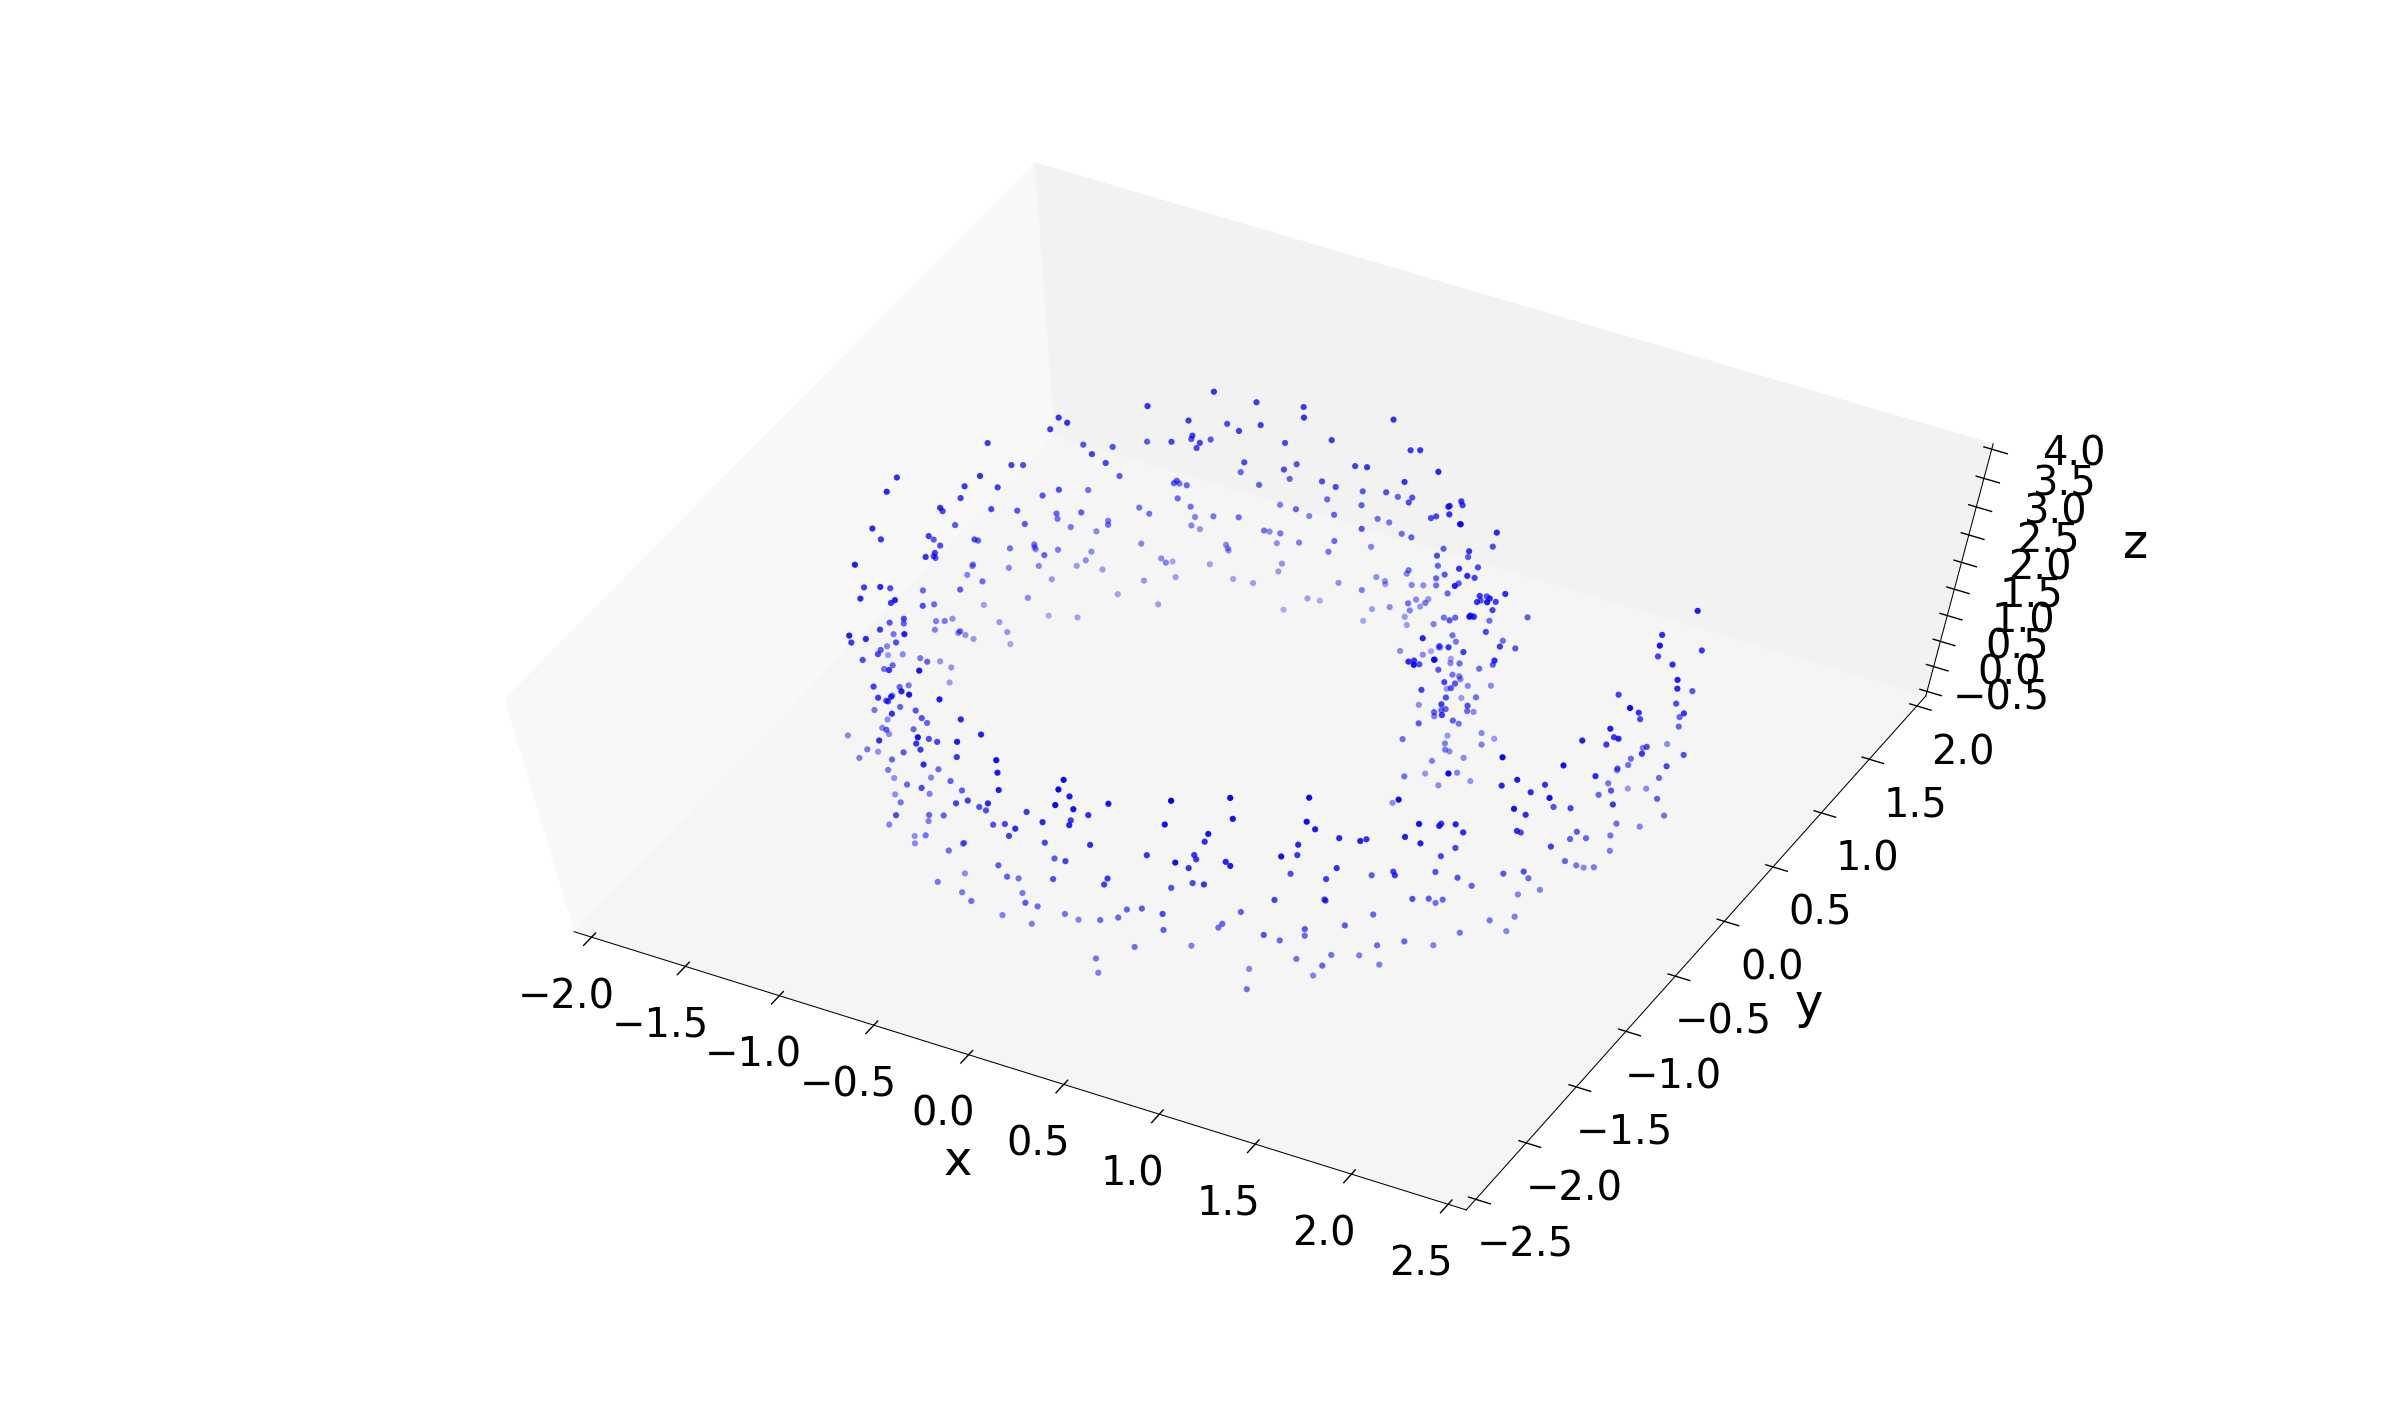
\includegraphics[width=1.0\textwidth]{dmaps_dataset}
      \caption{Three dimensional dataset lying on a curved surface.}
      \label{fig:swissroll}
  \end{subfigure}
  \begin{subfigure}{1.0\textwidth}
      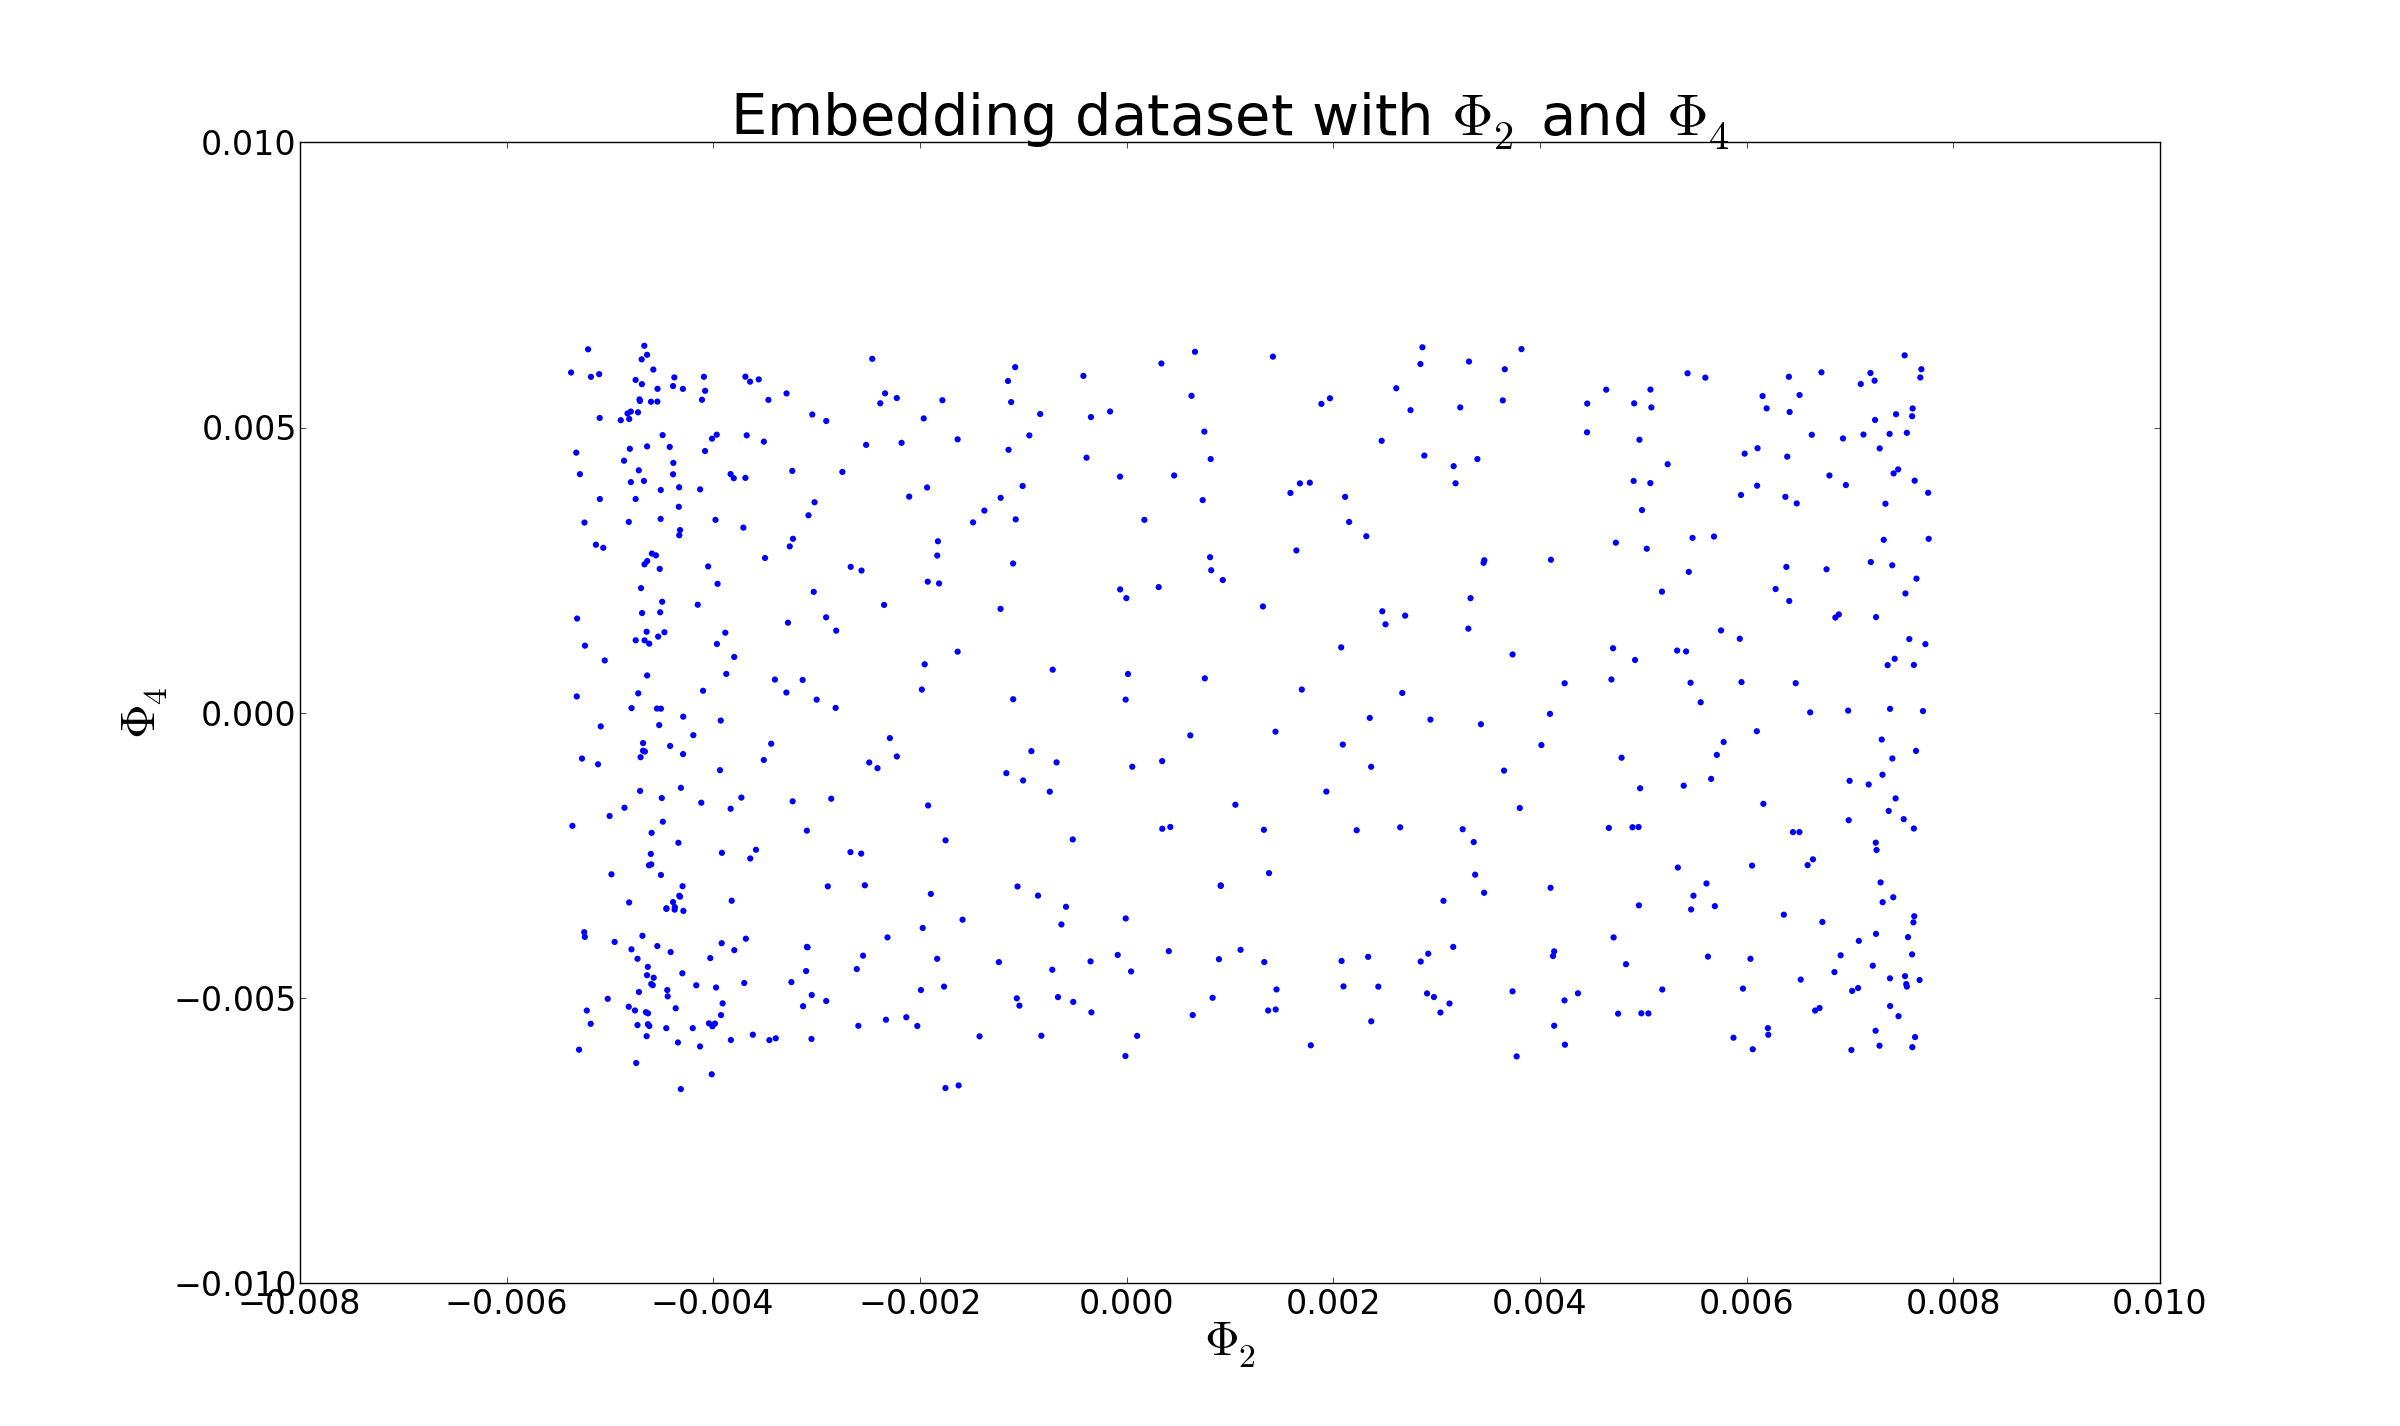
\includegraphics[width=1.0\textwidth]{dmaps_embedding}
      \caption{Embedding of data with first two unique DMAP coordinates. DMAP is able to uncover the underlying, nonlinear, two-dimensional parameterization of the datset.}
      \label{fig:swissroll:embedding}
  \end{subfigure}
    \end{center}
  \caption{Illustration of DMAPS ability to uncover nonlinear manifolds.}
\end{figure}

\clearpage


\section{Distances between data points}
In order to simulate diffusion over the dataset, DMAPS requires the distance between two points, $d(x_i, x_j) = \| x_i - x_j \|$, to be well defined. When each point $x_i$ is a vector in $\mathbb{R}^n$ as in our previous examples, the Euclidean distance between points is often sufficient. However, in the dataset we investigate below, each point $x_i$ is not a vector, but actually a graph (or network), denoted by $g_i$.

There are a number of ways of quantifying the distance between two graphs, $d(g_i, g_j)$, such as measuring how easily $g_i$ can be transformed into $g_j$, or by comparing random walks on the graphs \cite{edit_dist} \cite{graph_kernels}. In this paper, we consider two graphs to be similar if they share similar numbers of certain features. More precisely, we define a list of $k$ subgraphs $S=\{s_1, s_2, \ldots, s_k\}$, as shown in Fig. (\ref{fig:subgraph_counting}). We then record how many times each subgraph appears in our input graph in a vector $x_i = \{c_1^i, c_2^i, \ldots, c_k^i\}$, where $c_j^i$ is the number of times subgraph $s_j$ was found in input graph $g_i$. This process maps each graph to a vector of subgraph counts: $g_i \rightarrow x_i, \; \; x_i = \{c_1^i, c_2^i, \ldots, c_k^i\}$ in $\mathbb{R}^k$. We then use these vectors as the input to DMAPS, and use the Euclidean distance as our notion of similarity. Thus $d(g_i, g_j) = \| x_i - x_j \|_2$. A schematic illustrating this process is given in Fig. (\ref{fig:subgraph_counting}).

\section{Example problem}

We illustrate the application of DMAPS to a set of graphs using 

\begin{figure}[!h]
  \begin{center}
    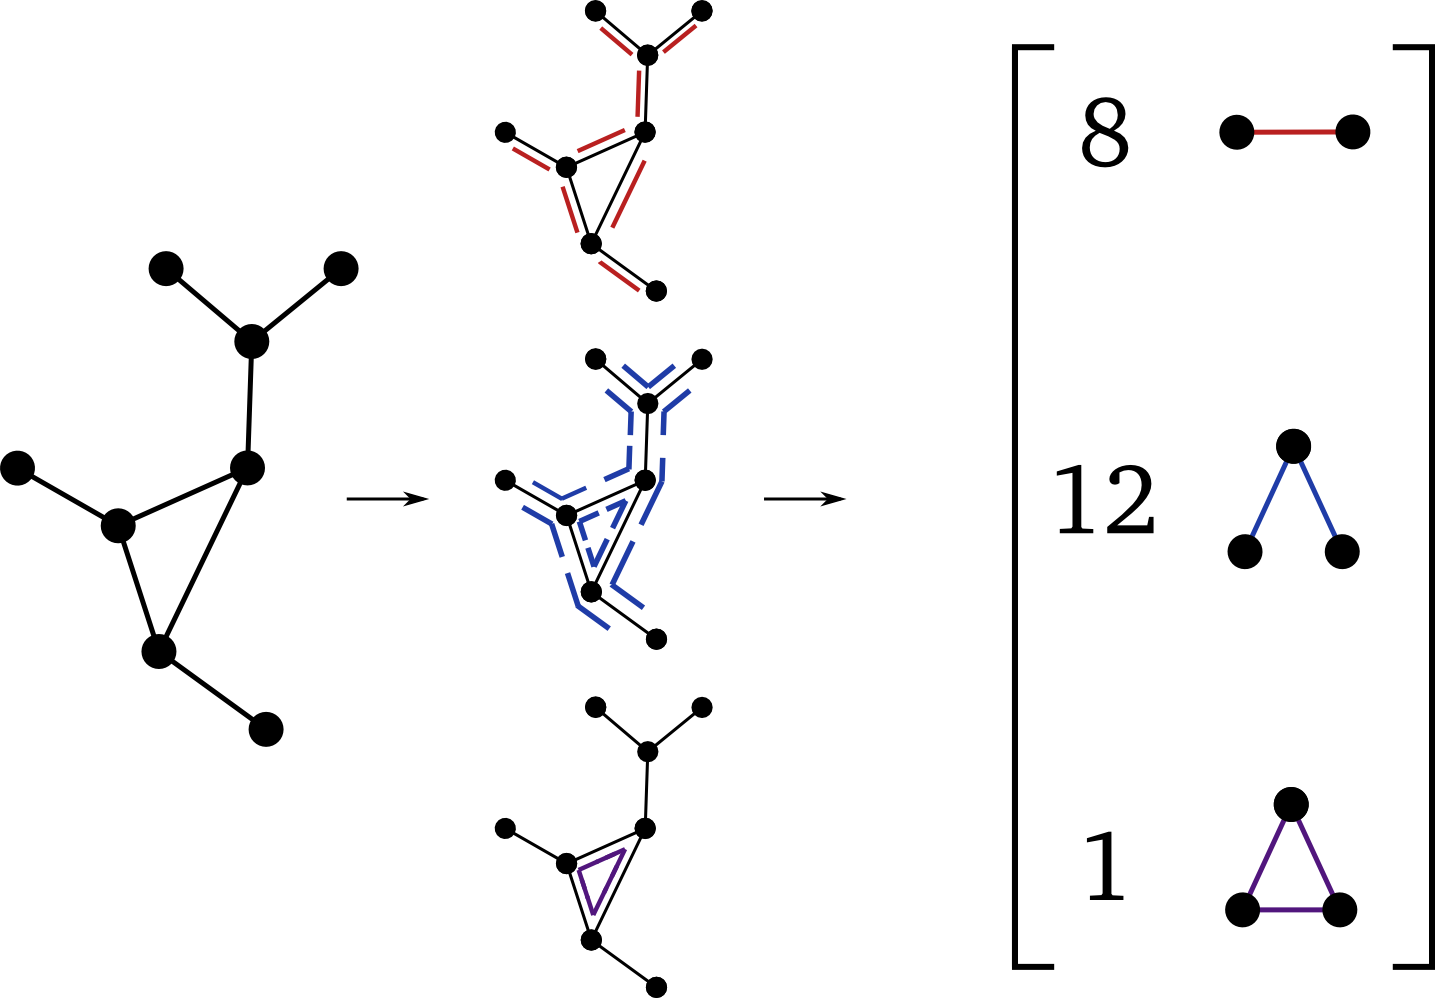
\includegraphics[width=0.6\textwidth]{subgraph_counting}
    \caption{Illustration of the subgraph-enumeration process with input graph $G$ and subgraph set $S$.}
  \end{center}
  \label{fig:subgraph_counting}
\end{figure}


\end{document}

